\section{SENSITIVITY ANALYSIS AND EXPERIMENTATION}

\subsection{Sensitivity Analysis}

To see the robustness of the model an sensitivity analysis was achieved. This procedure consists of a variation of some of the parameters of the model between $-10\%$ to $10\%$. 

The model, as explained before, some parameters where not able to be fitted because the data was too small. In this manner, we chose to see how the parameters of this elected distributions affected the output of the model. The result if this test is shown in Fig. \ref{fig:sens-anal}. 

\begin{figure}[H]
    \centering
    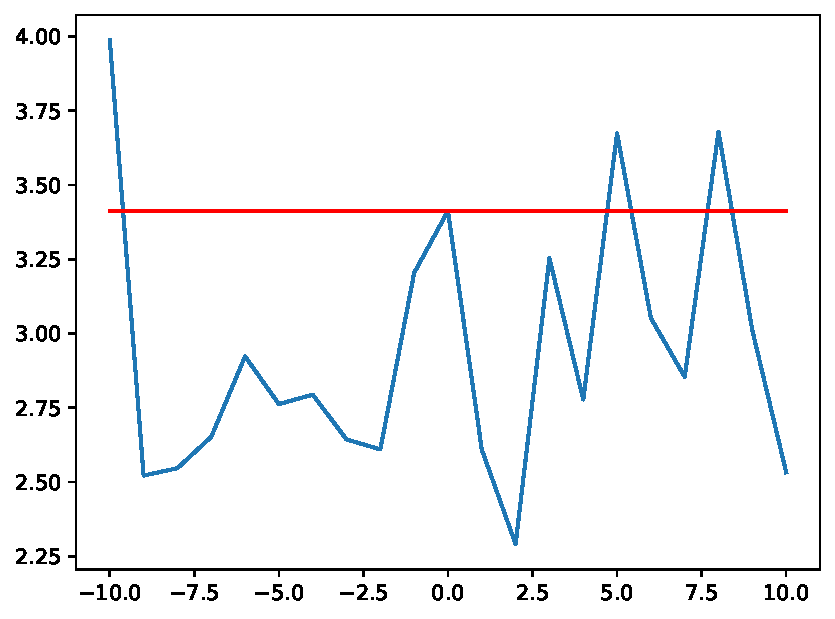
\includegraphics[scale=0.6]{files/sens-anal.pdf}
    \caption{Sensitivity analysis}
    \label{fig:sens-anal}
\end{figure}

It is seen that, although the simulation does change while changing the parameters of this distributions, this does not present a major problem as the output of the model does not change drastically. Hence, it is confirmed that the suppositions are not affecting in a damaging manner the simulation.

\subsection{Optimization}
The priority that each module attend (Table \ref{tab:pol_mod}) is not only is a key factor to consider in the queue logistics, but also a highly feasible strategy to implement in the real system since it only requires the adjustment on the queueing platform. The idea is to find the best combinations of priorities per (open) module to minimize the average queue time. The optimization scheme we propose takes the initial ``solution'', i.e. Table \ref{tab:sets_priorities_opt}, and apply a heuristic approach based on local search.

\begin{table}[H]
\centering
\begin{tabular}{ccl}
\hline
\textbf{Set} & \textbf{Amount} & \textbf{Priority} \\ \hline
1            & 1               & {[}10{]}          \\ 
2            & 1               & {[}4, 9, 5{]}     \\
3            & 1               & {[}4, 5, 9{]}     \\
4            & 2               & {[}7, 3, 8, 10{]} \\
5            & 4               & {[}3, 8, 7, 10{]} \\
6            & 5               & {[}3, 7, 8, 10{]} \\
\hline
\end{tabular}
\caption{Sets and priorities.}
\label{tab:sets_priorities_opt}
\end{table}

We use a standard Variable Neighborhood Search (VNS) \cite{hansen2006variable}, using classic neighborhood operators:
\begin{itemize}
\item In-Set Swap: Swaps two priorities within the same set (Figure \ref{fig:inset_swap}).
\begin{figure}[H]
    \centering
    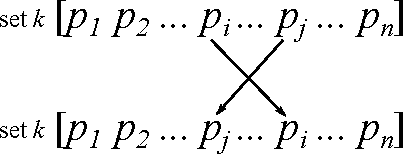
\includegraphics[scale=0.75]{files/inset_swap.pdf}
    \caption{In-set swap operator.}
    \label{fig:inset_swap}
\end{figure}
\item Best Insertion: Takes a node and attempts to find the best insertion within the set (Figure \ref{fig:best_ins}).
\begin{figure}[H]
    \centering
    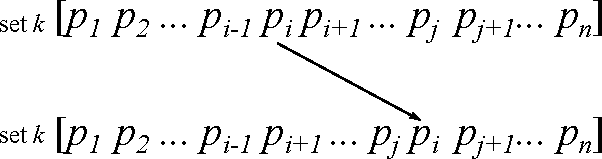
\includegraphics[scale=0.75]{files/bset_insert.pdf}
    \caption{Best-insertion in-set operator.}
    \label{fig:best_ins}
\end{figure}
\item Inter-Set Swap: Same as in-set, but attempting between two nodes in different sets (\ref{fig:inter_swap}).
\begin{figure}[H]
    \centering
    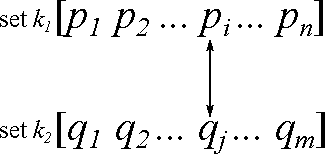
\includegraphics[scale=0.75]{files/interset_swap.pdf}
    \caption{Inter-set swap operator.}
    \label{fig:inter_swap}
\end{figure}
\end{itemize}

We refer to \cite{paraskevopoulos2008reactive} and \cite{fosin2014vehicle} for the local search operators. If the third operator swaps a priority into a set that already had that priority, one is chosen randomly and deleted. Otherwise, we assume that the number of priorities will not change, e.g. the number of appearances in all sets of policy ``3'' remains constant on each iteration and so forth.

After the optimization is done, an ANOVA test is performed in order to check if the mean of the output data is significantly improved after the optimization \cite[pp. 662-665]{wackerly2010estadistica}. 

The result of this heuristic is \ref{tab:optimal}. Furthermore, the evolution of the waiting time for the selected type of patient is shown in the Fig. \ref{fig:optimal}

\begin{table}[H]
\centering
\begin{tabular}{lll}
\hline
Set & Amount & Priority       \\ \hline
1   & 1      & {[}5,4,9{]}    \\
2   & 1      & {[}10{]}       \\
3   & 1      & {[}8,10,7,3{]} \\
4   & 1      & {[}7,3,10,8{]} \\
5   & 1      & {[}8,10,3,7{]} \\
6   & 1      & {[}3,7,8,10{]} \\
7   & 1      & {[}8,3,7,10{]} \\
8   & 1      & {[}7,8,3,10{]} \\
9   & 1      & {[}8,7,3,10{]} \\
10  & 1      & {[}10,7,3,8{]} \\
11  & 1      & {[}3,8,7,10{]} \\
12  & 1      & {[}7,3,8,10{]} \\ \hline
\end{tabular}
\caption{Found table of priorities.}
\label{tab:optimal}
\end{table}

\begin{figure}
    \centering
    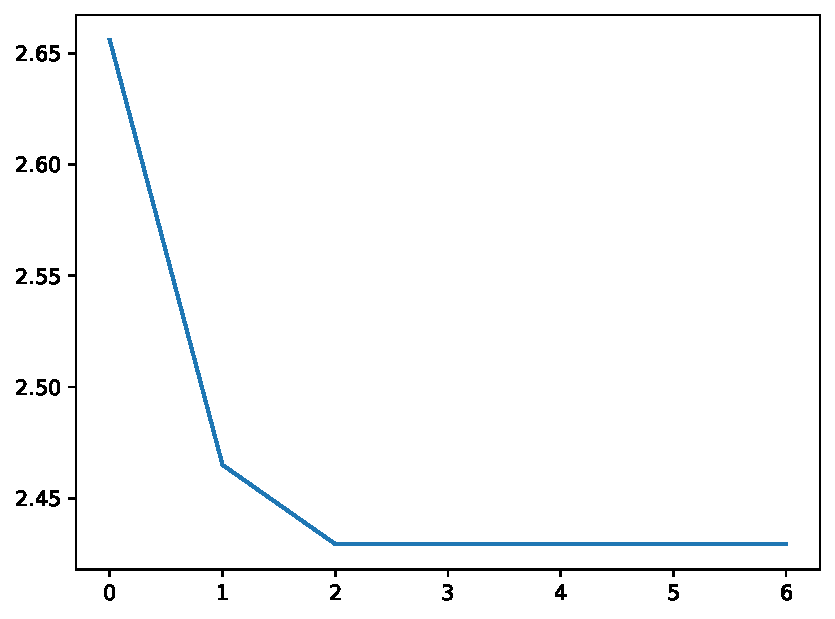
\includegraphics[scale=0.6]{files/opti.pdf}
    \caption{Waiting time for selected pacient changing over the iterations of VNS}
    \label{fig:optimal}
\end{figure}

It is important to notice that the best solution found was by using all the resources in all the different ways possible, so each one attend a different and unique priority. This is due to using all the resources to attend all the possible priorities, therefore reducing this waiting time.